% Fig 3.1 — End-to-end thesis pipeline
% Compile standalone:  xelatex fig_3_1_pipeline.tex
% Or copy the tikzpicture block into the thesis chapter.

\documentclass[border=4pt]{standalone}
\usepackage{tikz}
\usetikzlibrary{positioning, arrows.meta, shapes.geometric}

\begin{document}
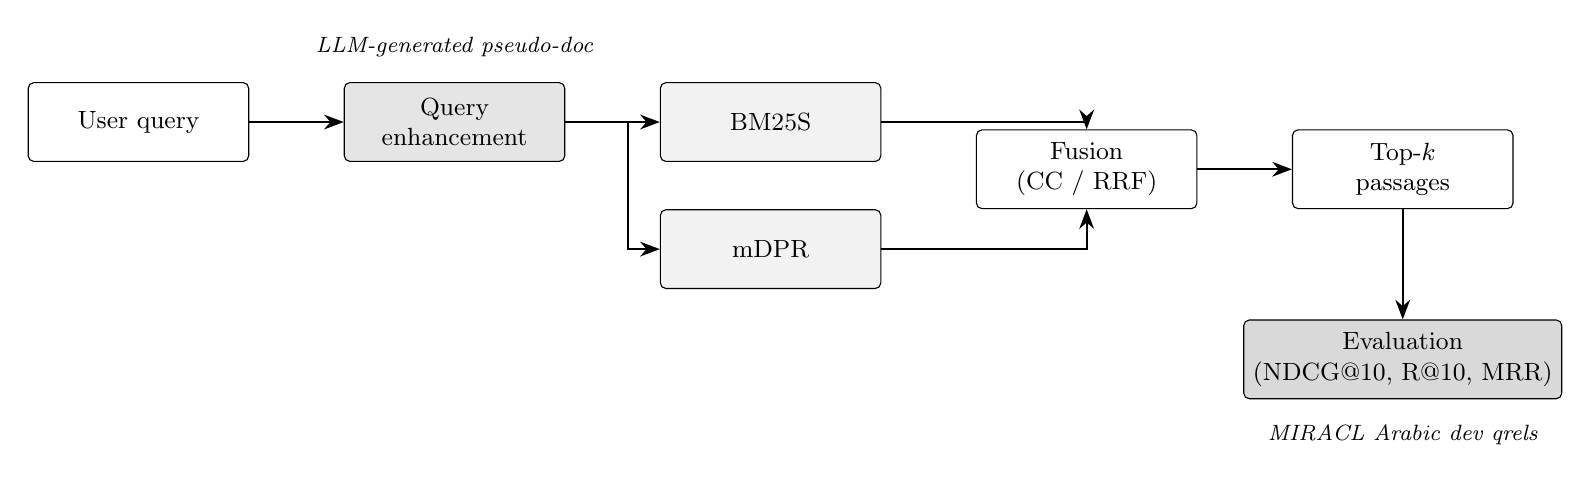
\begin{tikzpicture}[
    >=Stealth,
    node distance=14mm and 12mm,
    block/.style={rectangle, draw, rounded corners=2pt,
                  minimum width=28mm, minimum height=10mm,
                  align=center, font=\small},
    qe/.style={block, fill=black!10},
    retr/.style={block, fill=black!5},
    eval/.style={block, fill=black!15},
    arrow/.style={-{Stealth[length=2.5mm]}, thick}
]
  \node[block] (q) {User query};
  \node[qe, right=of q] (qe) {Query\\enhancement};
  \node[retr, right=of qe] (r1) {BM25S};
  \node[retr, below=6mm of r1] (r2) {mDPR};
  \node[block, right=of r1, yshift=-6mm] (fus) {Fusion\\(CC / RRF)};
  \node[block, right=of fus] (topk) {Top-$k$\\passages};
  \node[eval, below=of topk] (eval) {Evaluation\\(NDCG@10, R@10, MRR)};

  \draw[arrow] (q) -- (qe);
  \draw[arrow] (qe.east) -- ++(8mm,0) |- (r1.west);
  \draw[arrow] (qe.east) -- ++(8mm,0) |- (r2.west);
  \draw[arrow] (r1.east) -| (fus.north);
  \draw[arrow] (r2.east) -| (fus.south);
  \draw[arrow] (fus) -- (topk);
  \draw[arrow] (topk) -- (eval);

  \node[font=\footnotesize\itshape, above=2mm of qe] {LLM-generated pseudo-doc};
  \node[font=\footnotesize\itshape, below=2mm of eval] {MIRACL Arabic dev qrels};
\end{tikzpicture}
\end{document}
